\section*{Bài 1:}
Cho 4 điểm $A, B, C, D$ không cùng thuộc một mặt phẳng. Trên các đoạn thằng $AB, AC, BD$ lần lượt lấy các điểm $M, N, P$ sao cho $MN$ không song song với $BC$. Tìm giao tuyến của $(BCD)$ và $(MNP)$.
\begin{figure}[H]
\centering
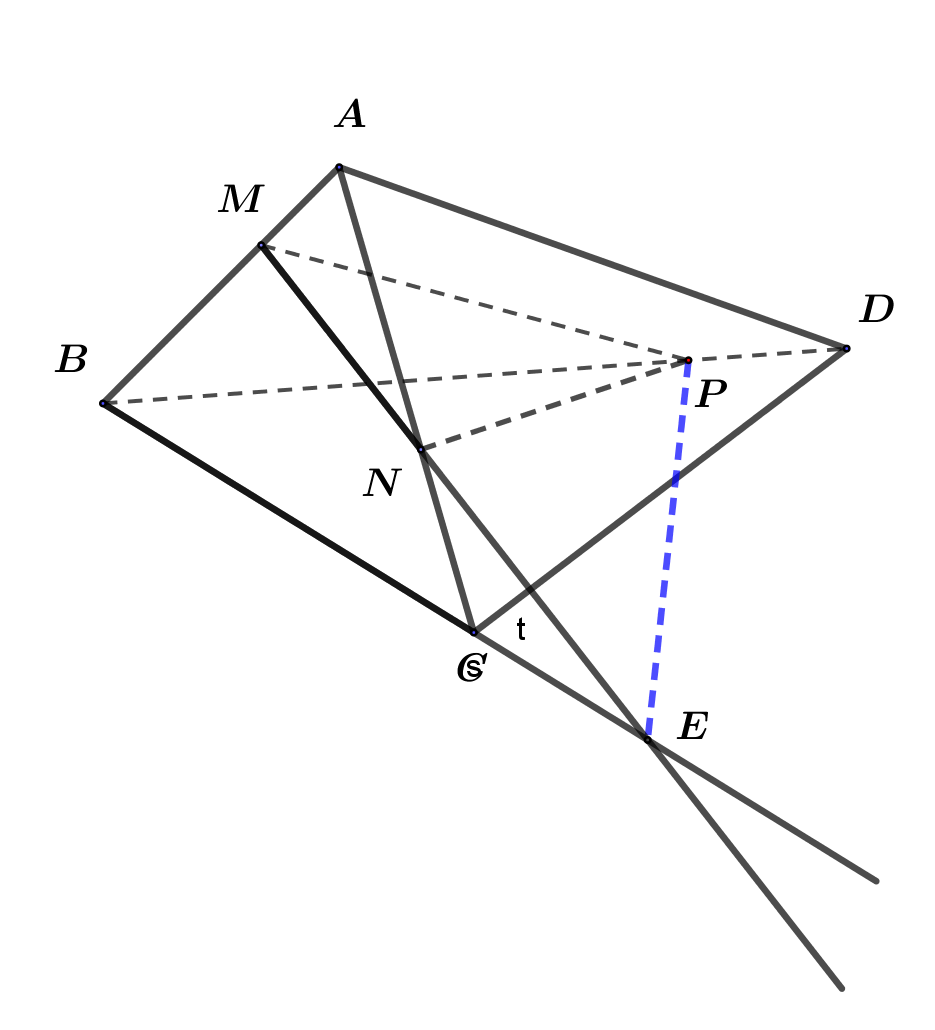
\includegraphics[width=6cm]{images/quizz1/quizz_1_figure.png}
\caption{Hình vẽ bài 1}
\end{figure}

\subsection*{Lời giải:}
\begin{itemize}
\item Ta có $P \in BD$ mà $BD \subset (BCD) \Rightarrow P \in (BCD)$ 
\item Mặt khác ta lại có $ P \in (MNP) $
\end{itemize}
$\Rightarrow P$ là điểm chung của $(BCD)$ và $(MNP)$

\vspace{5mm}
Trong mặt phẳng $(ABC)$ gọi $E = MN \cap BC$
\begin{itemize}
\item $ E \in BC$ mà $BC \subset (BCD) \Rightarrow E \in (BCD)$
\item $ E \in MN$ mà $MN \subset (MNP) \Rightarrow E \in (MNP)$
\end{itemize}
$\Rightarrow E$ là điểm chung của $(BCD)$ và $(MNP)$

\vspace{5mm}
Từ trên ta suy ra kết luận:
$PE$ là giao tuyến của 2 mặt phẳng $(BCD)$ và $(MNP)$